\section{Building \smt Systems} \label{sec:done}

Although the vision of stable multithreading is appealing, realizing it
faces numerous challenges.  Three main challenges are:

\begin{enumerate}

\item[$\bullet$] How can we compute the schedules to map inputs to?  The 
schedules
  must be feasible so executions reusing them do not get stuck.
  They should also be highly reusable.

\item[$\bullet$] How can we enforce schedules deterministically and
  efficiently?  ``Deterministically'' so executions that reuse a schedule
  cannot deviate even if there are data races, and ``efficiently'' so
  overhead does not offset reliability benefits.
  This challenge is also a decades-long challenge in the area of
  deterministic execution and replay.

\item[$\bullet$] How can we handle multithreaded server programs?  They often 
run for a
  long time and react to each client request as it arrives, making their
  schedules very specific to a stream of requests and difficult to reuse.

\end{enumerate}

Over the past four years, we have been tackling these challenges and
building \smt systems, which resulted in two \smt prototypes,
\tern~\cite{cui:tern:osdi10} and \peregrine~\cite{peregrine:sosp11}, that
frequently reuse schedules with low overhead.  This section describes our
solutions to these challenges.  Our solutions are by no means the only
ones; subsequent to \tern, others have also built a system that
stabilizes schedules for general multithreaded programs~\cite{dthreads:sosp11}.



\section{\tern: Computing Highly-reusable Schedules} \label{sec:tern}

%% how to collect schedules?
%% from dynamic executions
%% schedule memoization idea and advantages
%%
%% why precondition
%% example of pbzip:
%% results: frequently reuse schedules

Crucial to implementing \smt is how to compute the set of schedules for
processing inputs.  At the bare minimum, a schedule must be feasible when
enforced on an input, so the execution does not get stuck or deviate from
the schedule.  Ideally, the set of schedules should also be small for
reliability.  One possible idea is to pre-compute schedules using static
source code analysis, but the halting problem makes it undecidable to
statically compute schedules guaranteed to work dynamically.  Another
possibility is to compute schedules on the fly while a program is running,
but the computations may be complex and their overhead high.

Instead, we compute schedules by recording them from past executions; the
recorded schedules can then be reused on future inputs to stabilize
program behaviors.  \tern, our system implementing this idea, works as
follows.  At runtime, it maintains a persistent cache of schedules
recorded from past executions.  When an input arrives, \tern searches the
cache for a schedule compatible with the input.  If it finds one, it
simply runs the program while enforcing the schedule.  Otherwise, it runs
the program as is while recording a new schedule from the execution, and
saves the schedule into the cache for future reuse.

The \tern approach to computing schedules has several benefits. First, by
reusing schedules shown to work, \tern may avoid potential errors in
unknown schedules, improving reliability.  A real-world analogy is the
natural tendencies in humans and animals to follow familiar routes to
avoid possible hazards along unknown routes.  Migrant birds, for example,
often migrate along fixed flyways.  Why don't our multithreading systems
learn from them and reuse familiar schedules?  (The name \tern comes from
the Arctic Tern, a bird species that migrates the farthest among all
animals%~\cite{artic-tern-wiki}
.)

Second, \tern explicitly stores schedules, so developers and users can
flexibly choose what schedules to record and when.  For instance,
developers can populate a cache of correct schedules during testing and
then deploy the cache together with their program, improving testing
effectiveness and avoiding the overhead to record schedules on user
machines.  Moreover, they can run their favorite checking tools on the
schedules to detect a variety of errors, and choose to keep only the
correct schedules in the cache.

Lastly, \tern is efficient because it can amortize the cost of computing
schedules.
%recording and checking one schedule over many executions that reuse the
%schedule.
Specifically, recording and checking a schedule is more expensive than
reusing a schedule,
% because \tern has to track more things.  Fortunately, 
but, fortunately, \tern does it only once for each schedule and then
reuses the schedule on many inputs, amortizing the cost.

A key challenge facing \tern is to check that an input is compatible with
a schedule before executing the input under the schedule.  Otherwise, if
\tern tries to enforce a schedule, for instance, of two threads on an input
that requires four, the execution would not follow the schedule.  This
challenge turns out to be the most difficult one we must solve in building
\tern.  Our final solution leverages several advanced program
analysis techniques, including two new ones we
invent.  We refer interested readers to our
papers~\cite{cui:tern:osdi10,peregrine:sosp11} for details, and only
describe the high level idea here.

When recording a schedule, \tern tracks how the synchronizations in the
schedule depend on the input.  It captures these dependencies into 
a relaxed, quickly checkable set of
constraints called the \emph{precondition} of the
schedule.  It then reuses the schedule on all inputs satisfying the 
precondition,
avoiding the runtime cost of recomputing schedules.

A na\"ive way to compute the precondition is to collect constraints from
all input-dependent branches in an execution.  For instance, if a branch
instruction inspects input variable \v{X} and goes down the true branch,
we add a constraint that \v{X} must be nonzero to the precondition.  A
precondition computed this way is sufficient, but it contains many
unnecessary constraints concerning only thread-local computations.  Since
an over-constraining precondition decreases schedule-reuse rates, \tern
removes these unnecessary constraints from the precondition.

\begin{figure}[t]
\centering \tiny \lgrindfile{tern/code/pbzip2.cpp.lineno}
\caption{{\it An example program based on parallel compression utility
  \pbzip.}  It spawns \v{nthread} worker threads, splits a file among the
  threads, and compresses the file blocks in parallel.} \label{fig:pbzip2}
\end{figure}

\begin{figure}[t]
\centering
\begin{minipage}[c]{.9\linewidth}
\tiny \lgrindfile{tern/code/pbzip2-sync-order.cpp}
%\includegraphics[width=.4\textwidth]{figures/pbzip2-sync-order.eps}
\end{minipage}
\caption{{\it A synchronization schedule of the example program.}  Each
  synchronization is labeled with its line number in
  Figure~\ref{fig:pbzip2}.} \label{fig:pbzip2-sync-order}
\end{figure}

\begin{figure}[t]
\centering
\begin{minipage}[c]{0.6\linewidth}
\tiny \lgrindfile{tern/code/pbzip2-constraints.cpp}
\end{minipage}
\caption{{\it All input constraints collected for the schedule.}  Each
  constraint is labeled with its line number in
  Figure~\ref{fig:pbzip2}. Constraints collected from function
  \v{compress} are later removed by \tern because they have no effects on
  the schedule.  The remaining constraints simplify to
  $nthread=2$.} \label{fig:pbzip2-constraints}
\end{figure}

We illustrate how \tern works using a simple program based on the
aforementioned parallel compression utility \pbzip.
Figure~\ref{fig:pbzip2} shows this example. Its input includes all command
line arguments in \v{argv} and the input file data.
To compress a file, it spawns \v{nthread} worker threads,
splits the file accordingly, and compresses the file blocks in parallel by
calling function \v{compress}. To coordinate the worker threads, it uses a
synchronized work list. (Here we use work-list synchronization for
clarity; in practice, \tern handles Pthread synchronizations.) The example
actually has a bug: it is missing \v{pthread\_join} operations at line 7,
so the work list may be used by function \v{worker} after it is cleared at
line 8, causing potential program crashes. This bug is based on a real
bug in \pbzip.

We first illustrate how \tern records a schedule and its precondition.
Suppose we run this example with two threads, and \tern records a schedule
as shown in Figure~\ref{fig:pbzip2-sync-order}, which avoids the
use-after-free bug.  (Other schedules are also possible.)
% To record this schedule, \tern controls and records the synchronizations
% at lines 4, 6, 8, and 11.
To compute the precondition of the schedule, \tern first records the
outcomes of all executed branch statements that depend on input data.
Figure~\ref{fig:pbzip2-constraints} shows the set of constraints
collected.  It then applies advanced program analyses to remove the
constraints that concern only local computations and have no effects on
the schedule, including all constraints collected from function
\v{compress}.  The remaining ones simplify to $nthread=2$, which forms the
precondition of the schedule.  \tern stores the schedule and precondition
into the schedule cache.

We now illustrate how \tern reuses a schedule.  Suppose we want to
compress a completely different file also with two threads.  \tern will
detect that \v{nthread} satisfies $nthread=2$, so it will reuse the
schedule in Figure~\ref{fig:pbzip2-sync-order} to compress the file,
regardless of the file data.  This execution is reliable because the
schedule avoids the use-after-free bug.  It is also efficient because the
schedule orders only synchronizations and allows the \v{compress}
operations to run in parallel.  Suppose we run this program again with
four threads.  \tern will detect that the input does not satisfy the
precondition $nthread=2$, so it will record a new schedule and
precondition.

\subsection{\tern Evaluation} \label{sec:tern-eval}
In this section, we describe the main results of \tern, our first \smt
system.  We focus on two evaluation questions:

\begin{enumerate}

\item[\S\ref{sec:tern-stable}:] Can \tern frequently reuse schedules?  The
  higher the reuse rate is, the more stable program behaviors become, and
  the more efficient \tern is.

\item[\S\ref{sec:tern-efficient}:] Can \tern efficiently enforce schedules?  A
  low overhead is crucial for programs that frequently reuse schedules.

%% \item[\S\ref{sec:deterministic}:] Can \tern deterministically enforce
%%   schedules even if there are data races?  \tern is also deterministic,
%%   so it should preserve the benefits of determinism.

%% \item[\S\ref{sec:precise}:] Can \tern drastically improve the precision
%%   of sound program analysis?  The more precise, the more useful stable
%%   multithreading is at bettering program analysis.

%% \item[\S\ref{sec:annotation}:] Can \xxx significantly reduce manual
%%   annotation overhead?  Recall that our previous
%%   work~\cite{cui:tern:osdi10} required developers to manually annotate the
%%   input affecting schedules.

\end{enumerate}

We choose a diverse set of 14 programs as our evaluation benchmarks.
These programs are either widely used real-world parallel programs, such
as \apache and \pbzip, or parallel
implementations of computation-intensive algorithms in standard benchmark
suites.

\subsubsection{Stability} \label{sec:tern-stable}

\begin{table}[t]
\centering
\small
\begin{tabular}{lcc}
{\bf Program-Workload} & {\bf Reuse Rates (\%)} & {\bf Schedules} \\
\hline
\apache-trace          &   90.3\%    &    100      \\
\mysql-simple          &   94.0\%    &    50      \\
\mysql-tx              &   44.2\%    &    109      \\
\pbzip-usr             &   96.2\%    &    90      \\
\end{tabular}
\vspace{-.05in}
\caption{{\em Schedule reuse rates under four workloads.}  Column {\bf
    Schedules} indicates the number of schedules in the schedule cache.}
\label{tab:stability}
\vspace{-.05in}
\end{table}

We evaluate \tern's stability by measuring the schedule reuse rates under
given workloads.  Table~\ref{tab:stability} shows the results, obtained
from \tern.  The four workloads
are either real workloads collected by us or synthetic workloads used by the
developers themselves~\cite{cui:tern:osdi10}. %(\S\ref{sec:workloads}).
For three out of the four
workloads, \tern reuses a small number of schedules to process over
90\% of the workloads.  For \mysql-tx, \tern has a lower reuse rate
largely because the workload is too random to reuse schedules.
%% Second, we annotated only the SQL command as symbolic
%% without exposing the hidden states of MySQL (\S\ref{sec:window}) so that
%% we could measure \tern's performance in an adversarial setting
Nonetheless, it still processes 44.2\% of the workload.

\begin{figure}[t]
\centering
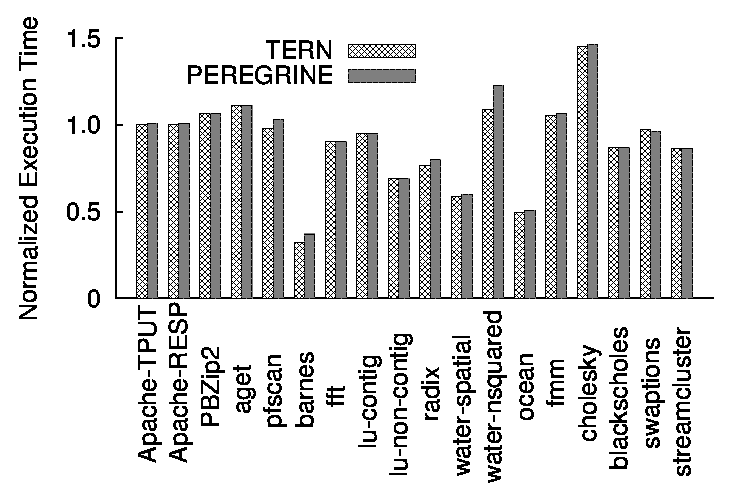
\includegraphics[width=.8\columnwidth]{tern/figures/overhead}
\vspace{-.3in}
\caption{{\em Relative overhead when reusing schedules.} } \label{fig:tern-overhead}
\vspace{-.05in}
\end{figure}


\subsubsection{Efficiency} \label{sec:tern-efficient}

Figure~\ref{fig:overhead} shows the relative overhead of \tern over
nondeterministic execution when reusing schedules, the smaller the better.  For seven out of
the fourteen programs, the replayer performed almost identically to
nondeterministic execution. For \pbzip and barnes, \tern performed
better.  This speedup came partially from the optimization to remove
unnecessary synchronizations~\cite{cui:tern:osdi10}.  \tern's overhead
for MySQL, volrend, raytrace, water-nsquared, and choleskey is relatively
large because these programs performed many synchronization operations
over a short period of time.  For instance, water-nsquared and cholesky
both call \v{pthread\_mutex\_lock()} and \v{pthread\_mutex\_unlock()} in a
tight loop.






\subsection{Peregrine} \label{sec:peregrine}
TBD



\section{Parrot} \label{ch:parrot}


%%\input{eval/eval}

%%\section{Model Checking} \label{sec:mc}
TBD.


